\section{COPPER Copper Colormap}

\subsection{Usage}

Returns a copper colormap.  The syntax for its use is
\begin{verbatim}
   y = copper
\end{verbatim}
\subsection{Example}

Here is an example of an image displayed with the \verb|copper|
colormap
\begin{verbatim}
--> x = linspace(-1,1,512)'*ones(1,512);
--> y = x';
--> Z = exp(-(x.^2+y.^2)/0.3);
--> image(Z);
--> colormap(copper);
\end{verbatim}
which results in the following image


\centerline{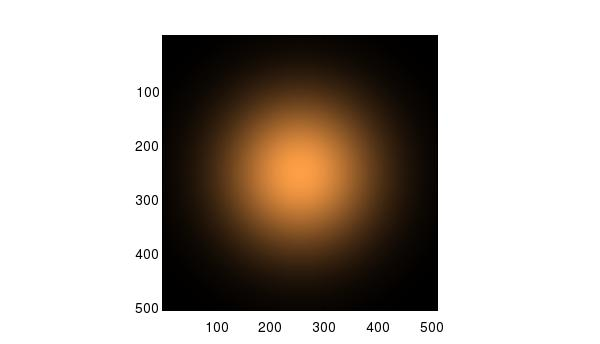
\includegraphics[width=8cm]{copper1}}

